\section{Pulsar Wind Nebulae Structure}
\seclabel{pwn_structure}


The basic picture of \acp{PWN}
comes from \cite{rees_1974_origin-magnetic} and
\cite{kennel_1984_magnetohydrodynamic-model}.  More 
sophisticated models have emerged over the years.  See, for example,
\cite{gelfand_2009_dynamical-model} and references therein.

The wind ejected from the pulsar's magnetosphere is initially
cold which means that it flows radially out from the pulsar.  This
unshocked pulsar wind only emits radiation through \ac{IC} scattering
\citep{bogovalov_2000_very-high-energy-gamma}.  This pulsar wind forms
a bubble as it presses into the \ac{SNR} and forms a termination shock
where the particle wind is further accelerated.

As the wind leaves the magnetosphere, it is believed to be dominated
by the energy carried off in electromagnetic fields (the pointing flux
\pointingflux).  The rest of the energy is released as a particle flux
(\particleflux).  We define the magnetization of the pulsar wind as
\begin{equation}
  \magnetization = \frac{\pointingflux}{\particleflux}
\end{equation}
Outside the pulsar light curve, typically $\magnetization>10^4$, but
at the termination shock typical values for $\sigma$ are $\lesssim0.01$
\citep{kennel_1984a_confinement-pulsars}.  The cause of this transition
is uncertain \citep{gaensler_2006_evolution-structure}.

\begin{figure}[htbp]
  \centering
    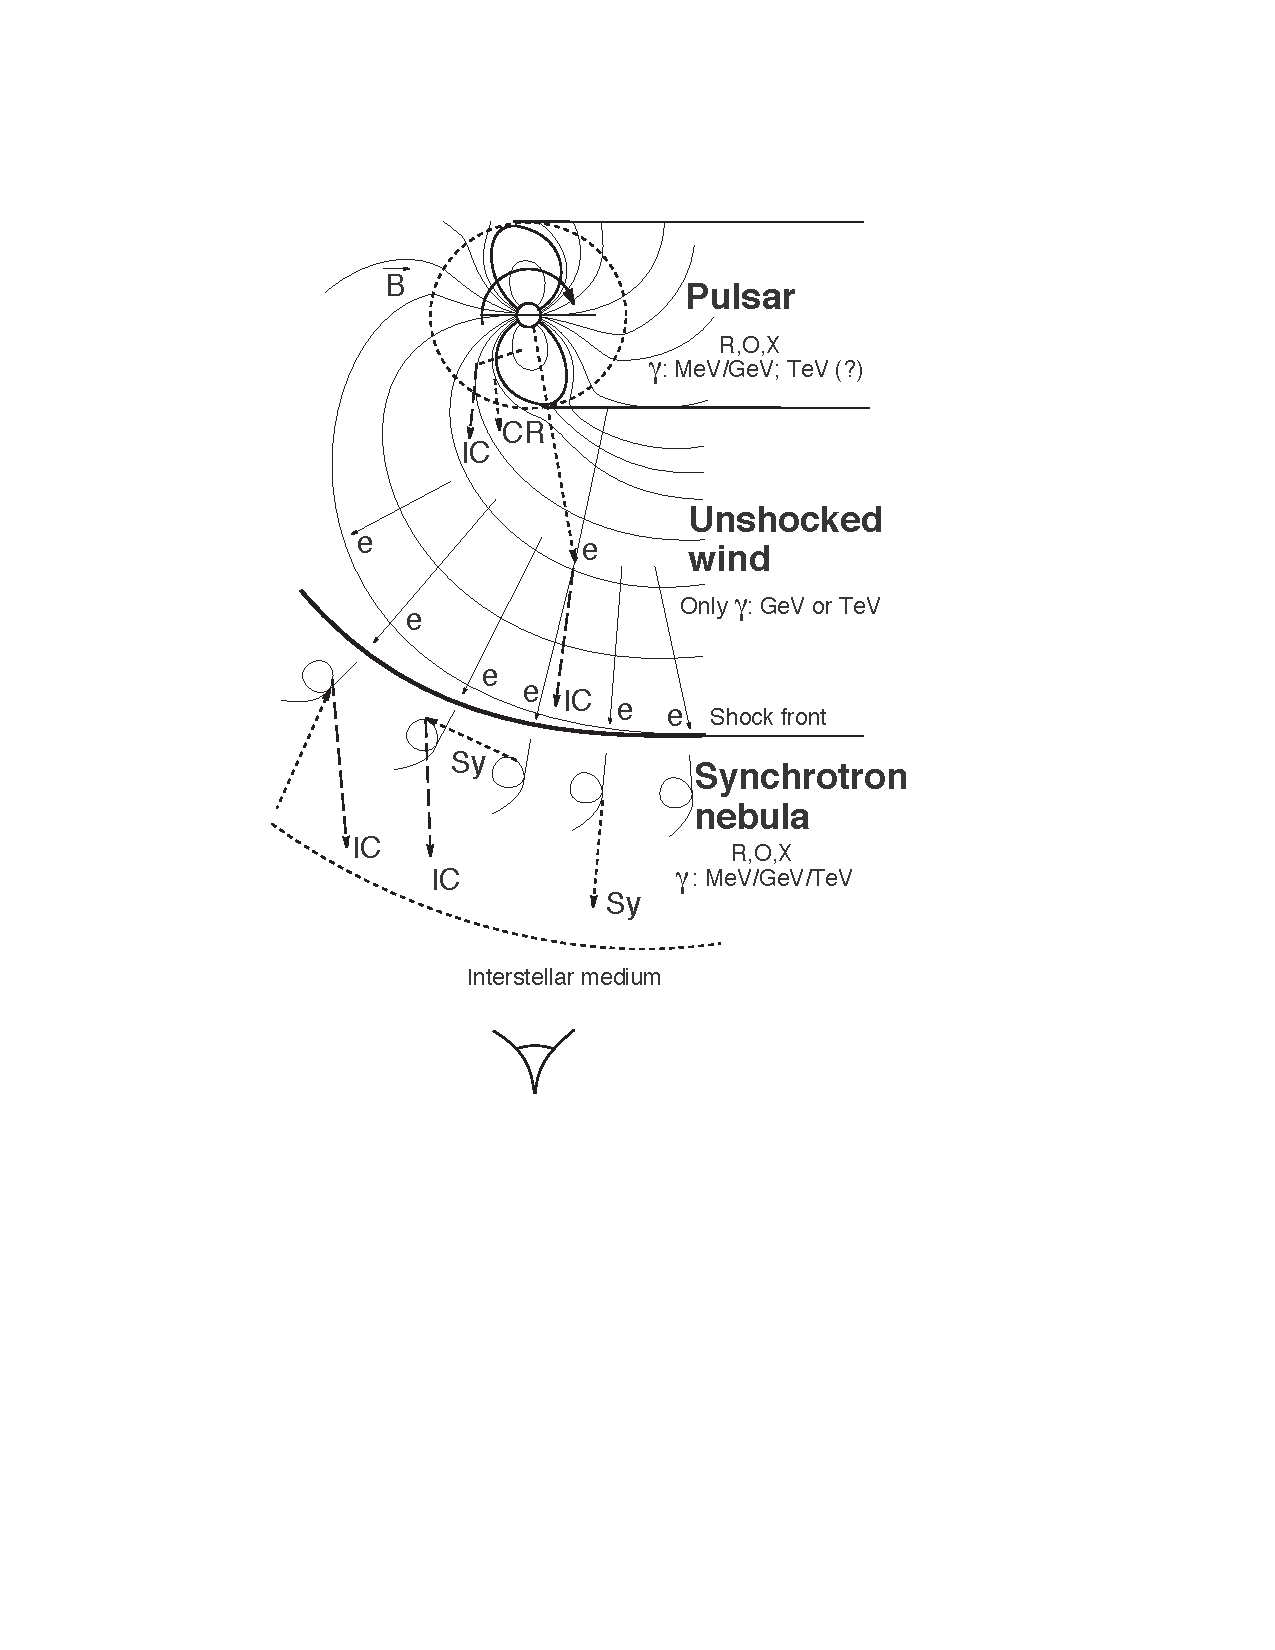
\includegraphics{chapters/pulsar_pwn_system/figures/termination_shock.pdf}
  \caption{The regions of emission in a pulsar/\ac{PWN} system. 
  This figure shows (top) the pulsar's magnetosphere, (middle), the
  unshocked pulsar wind and (bottom) the shocked pulsar wind which can
  be observed as the \ac{PWN}.
  ``R'', ``O'', ``X'', and ``$\gamma$'' describe sites of radio, optical, X-ray, and
  $\gamma$-ray emission respectively.
  ``CR'', ``Sy'', and ``IC'' refer to regions of curvature, inverse Compton, and
  synchrotron emission.
  Figure is taken from \cite{aharonian_2003_exploring-physics}.
  }
  \figlabel{termination_shock}
\end{figure}

The radius of the bubble (\radiusterminationshock) can be computed as the
radius where the ram pressure from the wind equals the pressure of the
gas in the \ac{SNR}.  The ram pressure is computed as the energy in the
bubble $\energydot \radiusterminationshock/c$ (assuming the particles
travel with a velocity $\approx \speedoflight$) divided by the volume
$4\pi\radiusterminationshock^3/3$: \begin{equation}
  \radiusterminationshock = \sqrt{\frac{\energydot}{\tfrac{4}{3}\pi \pressureISM \speedoflight}}.
\end{equation}
Here, \pressureISM is the pressure in the SNR.  Typical values
for the termination shock are 0.1\unitspace\parsec which is an
angular size $\sim$ \ac{arcsec} for distances $\sim\kiloparsec$
\citep{gaensler_2006_evolution-structure}.

At the termination shock, the particles are thermalized
(given a random pitch angle), and accelerated to energies of
$10^{15}\unitspace\electronvolt$ \citep{arons_1996_pulsars-gamma-rays}.
Downstream of the shock, the particles emit synchrotron and \ac{IC}
radiation as the thermalized electron population interacts with the
magnetic filed and seed photons \citep{gaensler_2006_evolution-structure}.
\figref{termination_shock} shows a diagram describing the pulsar
magnetosphere, the unshocked wind, and the synchrotron nebula which make
up the Pulsar/\ac{PWN} system.
